\section{Part 1: Modeling the Spread of Dandelions}

\subsection{Problem Analysis}
Because a dandelion is a living organism, its life follows a cycle through the several phases outlined in the previous section and in Figure~\ref{fig:dandelionlifecycle}. In addition to the cyclic nature of dandelion growth, some unpredictability exists due to changing environmental factors such as the wind and consumers. 

% So, we decided to model such factors with randomness because of the unpredictable nature of environmental and growth conditions.

%where the dandelion transforms from seed to puffball, is based on factors that change over time, including temperature, light, and nutrients. Once a dandelion reaches the puffball stage, those released seeds further contribute to the spread of dandelions.

\subsection {Assumptions}

\begin{table}[h]
\renewcommand{\arraystretch}{1.3}
    \begin{tabularx}{\textwidth}{lp{0.3\textwidth}X}
    \toprule
    \textbf{\#} & \textbf{Assumption} & {\centering \textbf{Justification}}  \\ \midrule
    
    \raggedright \nextassumption\label{assumption:1} & Dandelion seeds that land outside of the one-hectare plot of land will not be considered.  & The problem statement refers to a dandelion adjacent to a plot of land, so we interpreted that as modeling the growth of dandelions on that plot of land only. \\

    \rowcolor{gray!15} \raggedright \nextassumption\label{assumption:2} & Dandelion seeds behave mostly independently. & This allows us to develop an agent-based model to analyze each individual seed and easily adjust hyperparameters. \\

    \raggedright \nextassumption\label{assumption:3} & Although consumers are considered on the plot of land, human disturbances do not occur.  & Because information is not provided on the whereabouts of the plot of land, we assume that no humans will cause a significant disturbance to the growth of the dandelions. \\

    \rowcolor{gray!15} \raggedright \nextassumption\label{assumption:4} & No natural disasters will occur during the 12-month period we are modeling.  & Because the probability of a natural disaster occurring is low \cite{botzen_economic_2019}, our model does not consider it. \\

    \raggedright \nextassumption\label{assumption:5} & Nitrogen and potassium are the only nutrients affecting the growth of dandelions. & Higher potassium and nitrogen levels in the soil are the primary factors for increased seed germination and growth speed. \cite{noauthor_dandelion_nodate-2}.\\

    \rowcolor{gray!15} \raggedright \nextassumption\label{assumption:6} & Wind is the only factor that spreads the seeds from a puffball.  & As stated previously, no human disturbances could cause seeds to spread; therefore, wind is the only other natural factor that can affect seed dispersal. \\ 

    \raggedright \nextassumption\label{assumption:7} & Our model begins on January 1st, and ends on December 31st. & To model an entire year and include climate-related factors in our model, we are assuming that the first dandelion of the model exists on January 1st and is modeled until December 31st. \\ 

    \rowcolor{gray!15} \raggedright \nextassumption\label{assumption:8} & The one-hectare plot of land is square (100 meters by 100 meters). & By specifying the dimensions of the plot of land to be a square, we can better model the movement of dandelion seeds. \\ 
    \bottomrule
    
    \end{tabularx}
    
\end{table}

\subsection{Brief Overview}
First, we model the spread of the seeds from an initial puffball across a one-hectare plot of land. Afterward, we minimize the scope of the problem, focusing on each individual seed to model the independent growth of a seed. Once each seed matures into a puffball, the process repeats.

To model the life cycles of a seed, we developed a \textit{Seed Agent Model}, which considers environmental characteristics, such as wind, temperature, sunlight, and nutrients, to iterate each seed through a germination and plant growth life cycle. Finally, when new puffballs are fully developed, the Seed Agent Model is again applied to model the spread and growth of every new seed. Throughout our process, we incorporate environmental unpredictability by developing several stochastic processes. 

Below is a table of variables used throughout our agent-based model.

\begin{table}[h]
\renewcommand{\arraystretch}{1.3}
%p{0.8\linewidth
    \begin{tabularx}{\textwidth}{p{0.2\textwidth} lX}
    \toprule
    \textbf{Variable}           & \textbf{Symbol} & \textbf{Description}  \\ \midrule
    \raggedright Time Step & $t$  & Each time step is a day where \(t = 0\) is January 1 of a year. \\
    \rowcolor{gray!15}
    \raggedright Number of Moves & $N$  & Number of moves a seed takes in movement process. \\
    Coordinate Shift & $\Delta x, \Delta y$    &  Change in \(x\) or \(y\) coordinate of a seed in every move.  \\
    \rowcolor{gray!15} \raggedright  Death Date & $D$               &  Time of death of a seed, sampled from Exponential distribution.  \\
    \raggedright Plant Growth & $G$ & The stage of growth of a dandelion plant between 0 and 1. \\
    \rowcolor{gray!15} \raggedright Temperature Index & $T_I$ & A standardized metric to describe optimal temperatures for dandelions. \\
    \raggedright Light Index & $L_I$ & A standardized metric to describe optimal light levels for dandelions. \\
    \rowcolor{gray!15} \raggedright Nutrition Index & $N_I$ & A standardized metric to describe optimal soil conditions for dandelions. \\
    \bottomrule
    \end{tabularx}
\end{table}

\subsection{The Way Of The Wind: A Seed Dispersal Process}

We first identified the primary contributing factor of dandelion seed movement to be the wind \cite{wang_separating_2021}, following Assumption~\ref{assumption:6}. Thus, we decided to use the Brownian Motion Process to model the spread of dandelion seeds. Brownian Motion stochastic processes are often utilized to model the stochastic, or random, movement of particles in a particular medium, such as seeds in open air.

To begin, we define the number of seeds of the initial puffball dandelion to be \(S_0\). The puffball releases its \(S_0\) seeds into a \textit{stochastic Brownian motion process} in a 2D plane. 

To mimic the random nature of wind in determining a seed's new position, each seed will complete two stages of an algorithm. First, a seed is assigned a random number of position translations, or "moves." Next, the distance the seed moves in that position is randomly determined for each position translation. This allows us to model the varying movements of the dandelion seeds in all directions.

\subsubsection{Number of "Moves" a Seed Performs}
    First, we determine \(N\), the number of "moves" a seed will perform on the 2D plane in time-step \(t\). Next, we use a probabilistic model to account for varying winds in different climates and days. Therefore, we assign the random variable \(N\) with a non-homogeneous (changing over time) Poisson distribution and wind strength hyperparameter \(m(t)\), denoting the mean number of steps at time step \(t\). Poisson probability distributions are used when finding the number of events that occur in a given time frame. We can model this as 

    \begin{align}
        N & \sim \text{Poisson}(m(t)) \\
        \mathbb{P}(N=n) & = e^{-m(t)}\frac{\left[m(t)\right]^2}{n!} \nonumber
    \end{align}

    In other words, the number of moves a seed will take will be sampled from this Poisson distribution, which changes according to wind levels (Note: wind levels change based on the region and time). We use \(k\) to denote the \(k\)'th move out of \(n\) moves such that \(k \in [0, n]\).

\subsubsection{Distance Per "Move"}

    Next, we determine the change in position for each move \(k\). The seed will move a specified distance \(\Delta x\) and \(\Delta y\) which are sampled from a \(\text{Normal} (0, \sigma^2)\) such that the new coordinate for each seed after step \(k\) will be 

    \begin{equation}
        (x_i, y_i)_{k+1} = (x_i, y_i)_k + (\Delta x, \Delta y)
    \end{equation}

    \begin{align}
        \Delta x \text{ or } \Delta y & \sim \text{Normal}(0, \sigma^2) \\
        \mathbb{P}(\Delta x \text{ or } \Delta y = d) & = \frac{1}{\sigma \sqrt{2\pi}}e^{-\frac{1}{2}\left( \frac{d}{\sigma}\right)^2} \nonumber
    \end{align}
    
Recall that from Assumption~\ref{assumption:1}, dandelion seeds that travel outside our provided hectare of land are removed from the consideration of our model to simplify our model's scope.

\subsection{Race the Clock: Beating a Death Date}
After the seed is assigned a new location, the seed will go through two critical processes: (a) germination and (b) plant growth. However, the seed may die of natural causes before each phase. To account for this nuance, we introduce a \textit{Death Date} for each seed that resets at the end of the germination and plant growth stage. 

The first death date of a seed will be assigned after it lands on the ground and before it begins the germination process. The death date is determined by randomly sampling from a probabilistic survivorship curve (see Figure \ref{fig:exponentialdistribution}). If the seed successfully germinates before its assigned death date, it will be assigned a new death date for the plant growth cycle. 

\begin{figure}[h!]
\centering
    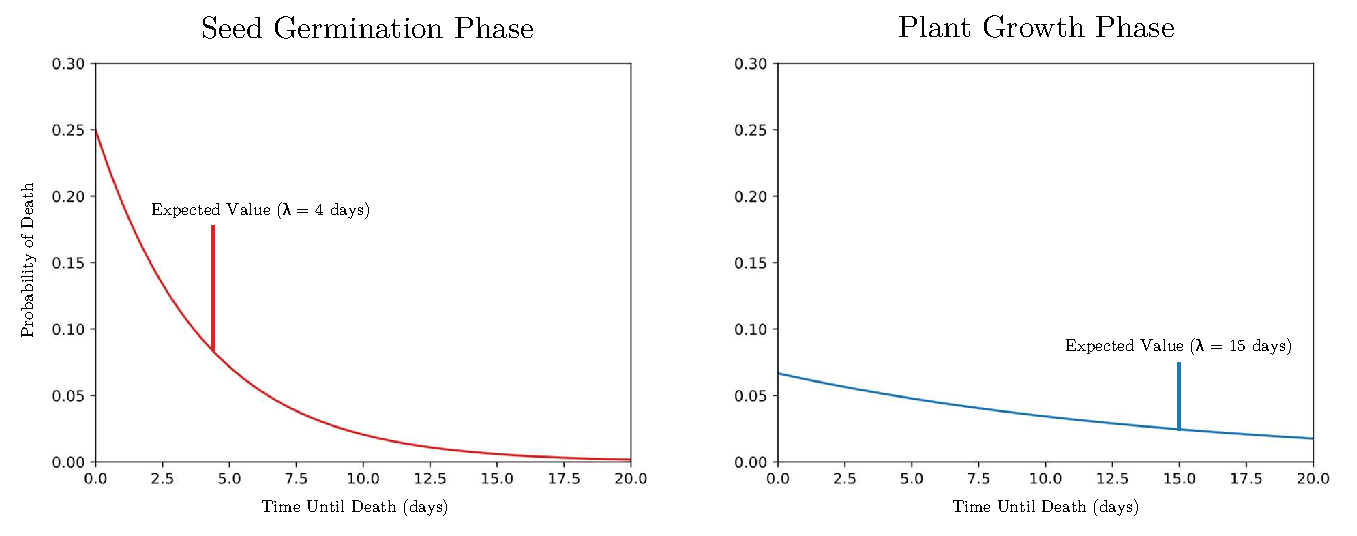
\includegraphics[scale=0.65]{figures/exponentialdistribution.pdf}
    \captionsetup{width=0.9\textwidth}
    \caption{\textbf{The survival rate of a seed during two major phases.}}
    \label{fig:exponentialdistribution}
\end{figure}

The survival rate of dandelions is often classified as a Type III survivorship curve \cite{noauthor_53_nodate}, where shorter lifespans are more probable than longer lifespans. Thus, due to the low percentage of seeds that eventually germinate, it is more likely to randomly select a relatively earlier death date than a later death date \cite{noauthor_dandelion_nodate-2}. 

Henceforth, we used a non-homogeneous (time-varying) Exponential distribution to model survival rates. However, per Assumption~\ref{assumption:2}, the only time dandelions are not independent is when two seeds land in the same place, thereby eliminating one of the two.

The probability of the random variable of seed death date \(D\) at time \(t\), \(\mathbb{P}(D = t)\), can be determined by finding the \textit{survivorship curve} of dandelions in their respective environments. 

\begin{align}
    D & \sim \text{Exponential}(\lambda(t)) \nonumber  \\
    \mathbb{P}(D = t) & = \lambda(t) e^{-\lambda(t) t}
\end{align}

where \(\frac{1}{\lambda(t)}\) is the average lifespan of a dandelion seed at time step \(t\). For regional calibration, \(\lambda(t)\) can be adjusted. For the sake of differentiating the death date of seeds and dandelion plants, we will introduce two hyperparameters \(\lambda_s(t)\) and \(\lambda_d(t)\) for the two stages, respectively \cite{board_of_pesticides_control_maine_dacf_dandelion-taraxacum_nodate}. Note that because no natural disasters nor human disturbances will occur on our hectare plot of land (Assumptions~\ref{assumption:3} and~\ref{assumption:4}), neither of these lifespan hyperparameters will be arbitrarily low.

\subsection{Stages of Dandelion Growth}

After a dandelion has landed in the ground and a death date has been assigned, we begin to model the dandelion growth process. There are two phases: (1) seed germination and (2) the plant growth process.

Because the seed germination stage is relatively shorter than the much longer plant growth process, we use historical data to determine a germination length and a more extended process to model the plant development cycle.

\subsubsection{Phase 1: Seed Germination}

To obtain the time for a seed to germinate, we sample from a \(\text{Normal } (\mu_{\text{germination}}(t), \sigma^2)\) distribution. Note that the mean duration of seed germination varies with regard to the climate and region \cite{board_of_pesticides_control_maine_dacf_dandelion-taraxacum_nodate}. Because seeds usually have different expected lifespans than dandelion plants, we assign a new death date from the seed survival distribution with a new hyperparameter \(\lambda_d(t)\) after every seed germination.

\subsubsection{Phase 2: Plant Development}

Once germinated, we define the growth function \(G\) based on three indices \(T_I\), \(L_I\), and \(N_I\) for temperature \(\tau(t)\), light levels \(l(t)\), and soil nutrient composition, respectively. When growth \(G\) is at 0, we say that a single dandelion just began growing (or germinating). When the growth \(G\) is at 1, we say that the dandelion is at the "puffball" stage and releases its seeds.

\begin{quote}
\textbf{Temperature Index}

For the \textit{temperature index} \(T_I: \tau(t) \longrightarrow [-1, 1]\), we define a piecewise function that assigns a negative score if the temperature (\(^\circ\)F) \(\tau(t)\)  falls out of the ideal dandelion growth temperatures and a positive score if the temperatures are ideal.  Positive scores are based on squared Euclidean distance from optimal temperatures \([50\hspace{0.1cm}^\circ\text{F},  77\hspace{0.1cm}^\circ\text{F}]\) \cite{board_of_pesticides_control_maine_dacf_dandelion-taraxacum_nodate}. Non-ideal temperatures are normalized on a logistic curve, allowing us to scale scores between -1 and 1, while adding a non-linearity factor to weigh the optimal values more heavily. So, we can define \(T_I\) as
\begin{align}
    T_I = 
    \begin{cases}
        \frac{-2}{1+e^{-0.1(\tau(t)-77)}} + 1, \hspace{2cm} & \tau(t) \geq 77 \\
        1 - \frac{1}{63.5^2} (\tau(t) - 63.5), & 50 < \tau(t) < 77 \\
        \frac{-2}{1+e^{-0.1(50-\tau(t))}} + 1, \hspace{2cm} & \tau(t) \leq 50\\
    \end{cases}
    \label{eq:tempindex}
\end{align}

\textbf{Light Index}

For the \textit{light index} \(L_I: l(t) \longrightarrow [-1, 1]\), we again define a piecewise function which similarly assigns scores but for the optimal interval of light hours \([6 \text{ hours}, 24 \text{ hours}]\)\cite{stewart-wade_biology_2002}. So, we define \(L_I\) as,

\begin{align}
    L_I = 
    \begin{cases}
        \frac{-2}{1+e^{-0.5(l(t)-24)}} + 1, \hspace{2cm} & l(t) \geq 24 \\
        1 - \frac{1}{15^2} (l(t) - 15), & 6 < l(t) < 24 \\
        \frac{-2}{1+e^{-0.5(6-l(t))}} + 1, \hspace{2cm} & l(t) \leq 24 \\
    \end{cases}
    \label{eq:lightindex}
\end{align}

\textbf{Nutrition Index}

Lastly, we define the soil \textit{nutrition index} \(N_I: (k(t),n(t)) \longrightarrow [-1, 1]\) to be a function on potassium levels and nitrogen levels (see Assumption~\ref{assumption:5}) in a given region where potassium and nitrogen levels are optimally between \([40, 80]\) and \([20, 40]\) ppm, respectively \cite{arizona_guide_nodate}. Based on this information, we formulate the following exponential transformation for the soil nutrient index. By defining a similar shape to the previous index functions and min-max scaling \(k(t)\) and \(n(t)\), we arrive at the following index function.

\begin{align}
    N_I = \exp\left(-\left(\frac{k(t)-60}{40}\right)^2\right) + \exp\left(-\left(\frac{n(t)-30}{30}\right)^2\right) - 1
    \label{eq:nutritionindex}
\end{align}
\end{quote}


Using the three indices from above (Equations~\ref{eq:tempindex},~\ref{eq:lightindex},~\ref{eq:nutritionindex}), we formulate the change in growth, \(\frac{dG(}{dt}(t)\) at time step \(t\) by scaling the sum of \(T_I\), \(L_I\), and \(N_I\) to match the time to fully grow a dandelion under optimal conditions (minimum 50 days) \cite{gardeningknowhowDandelionHarvest}. Furthermore, we scale the sum of the indices by \(\frac{1}{3}\) to return to the -1 to 1 scale, and another \(\frac{1}{50}\) as optimal growing conditions (minimum 50 days) would result in \(\frac{dG}{dt} = \frac{1}{50}\). Therefore, we define \(\frac{dG}{dt}(t)\) as,

\begin{align}
    \frac{dG}{dt}(t) = \frac{1}{3 \cdot 50}\left(T_I+L_I+N_I\right) \\
    \text{where } \max\left(\frac{dG}{dt}\right) = \frac{1}{50} \nonumber
\end{align}

\begin{figure}[h!]
\centering
    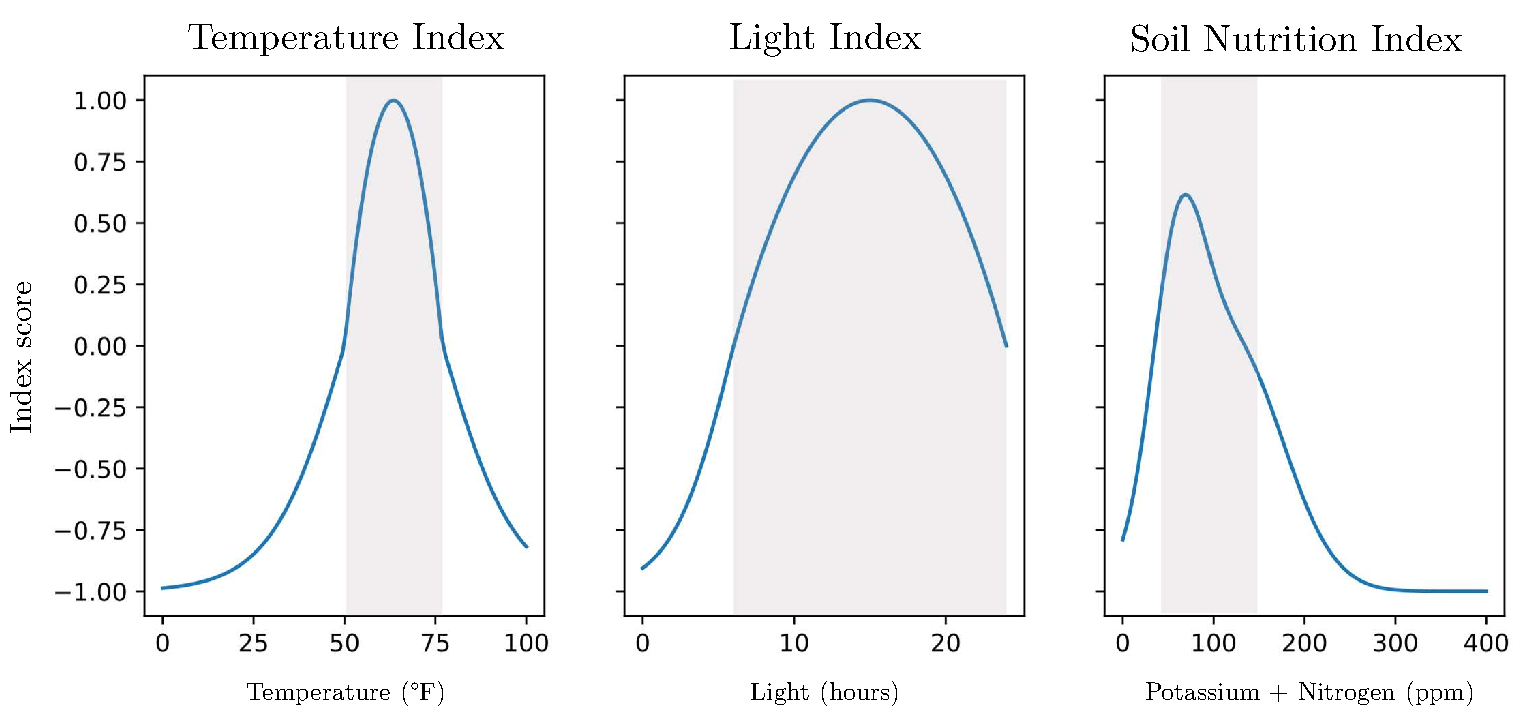
\includegraphics[scale=0.5]{figures/scoreindex.pdf}
    \captionsetup{width=0.9\textwidth}
    \caption{\textbf{From the left to right: \(T_I, L_I, N_I\) scores for plant growth.} Each shaded area represents the optimal interval for each unit of measure, which receives a positive score.}
    \label{fig:indexscoregraphs}
\end{figure}

\subsection{Seed Agent Model Overview}

Our method of modeling the spread of dandelions from an agent-based perspective is summarized in Figure~\ref{fig:partadiagram}.

\begin{figure}[h!]
\centering
    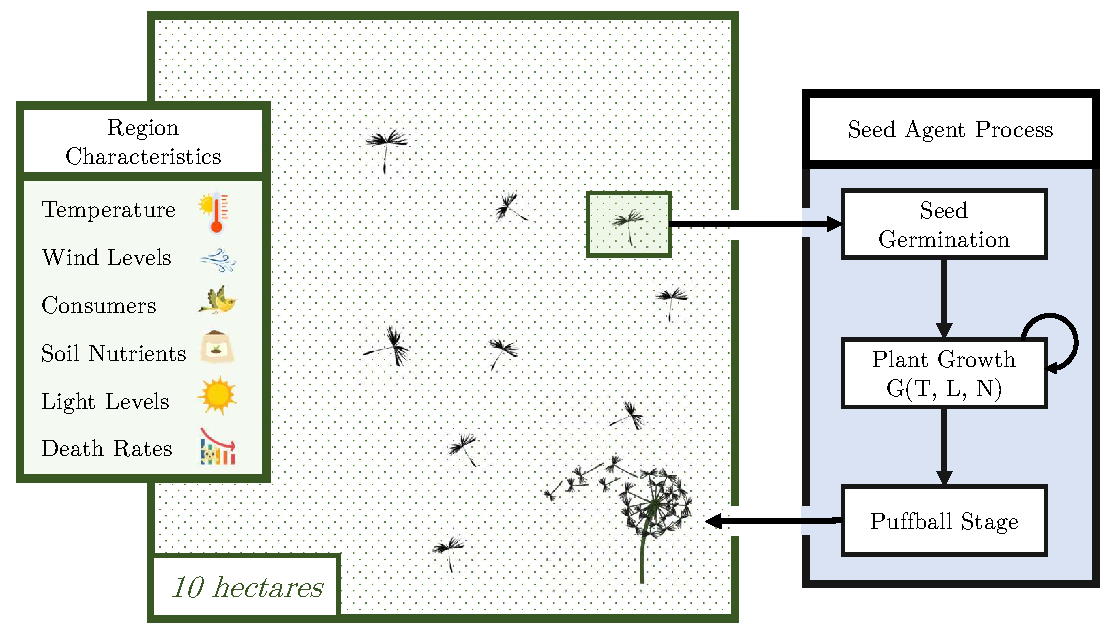
\includegraphics[scale=0.8]{figures/seedspreadprocess2.pdf}
    \captionsetup{width=0.9\textwidth}
    \caption{\textbf{Overview diagram of seed spread modeling.} }
    \label{fig:partadiagram}
\end{figure}